\documentclass[a4paper]{article}

\usepackage{geometry}                   % Disable paragraph indent.
    \setlength\parindent{0pt}           % Change page size to MS Word.
    \newgeometry{vmargin={25.4mm}, hmargin={27mm,27mm}}

% \usepackage[giveninits=true, sorting=none, url=false, isbn=false, citestyle=numeric-comp]{biblatex}
%     \renewbibmacro{in:}{}               % Bibliography (always use FULL path).
%     \addbibresource{/home/anton/Downloads/bib/PhD.bib}

\usepackage{amsmath}                    % Add AMS Math/Math tools.
\usepackage{upgreek}                    % Add non-italic Greek characters.

\usepackage{hyperref}                   % Add URLs.
% \usepackage[dvipsnames,table]{xcolor}   % Add colored text.
% \usepackage{standalone}                 % Allows for /input of other .tex file.
% \usepackage{seqsplit}                   % Allows splitting of protein sequences.

\usepackage{graphicx}                   % Enables images.
\usepackage{caption}                    % Enables advanced captions.
% \usepackage{multirow}                   % Enables multiple rows for images.
% \usepackage{subfig}                     % Enables multiple images.

\usepackage{xcolor}

\title{FDD3258 Assignment 1}
\date{\today}
\author{Anton Jansen, Michele Pellegrino}

\begin{document}

\maketitle

\section{Modeling sparse matrix-vector multiply}

\begin{enumerate}
    \setlength\itemsep{0.01em}
    \item If we do not consider data movement, we compute performance based on FLOPS and CPU speed i.e. $t = \text{nnz} \times 2c$ for our code. On my local machine (Ryzen 7 3800X @ 3.9 GHz):
    \begin{itemize}
        \setlength\itemsep{0.01em}
        \item $\text{nrows} = 10^2 \Rightarrow \text{nnz} = 5 \times 10^2 \Rightarrow t = (5 \times 10^2)(2)(3.9\times 10^9)^{-1} = 2.56 \times 10^{-7} \ \text{s}$
        \item $\text{nrows} = 10^4 \Rightarrow \text{nnz} = 5 \times 10^4 \Rightarrow t = (5 \times 10^4)(2)(3.9\times 10^9)^{-1} = 2.56 \times 10^{-5} \ \text{s}$
        \item $\text{nrows} = 10^6 \Rightarrow \text{nnz} = 5 \times 10^6 \Rightarrow t = (5 \times 10^6)(2)(3.9\times 10^9)^{-1} = 2.56 \times 10^{-3} \ \text{s}$
        \item $\text{nrows} = 10^8 \Rightarrow \text{nnz} = 5 \times 10^8 \Rightarrow t = (5 \times 10^8)(2)(3.9\times 10^9)^{-1} = 2.56 \times 10^{-1} \ \text{s}$
    \end{itemize}
    \item \begin{itemize}
          \setlength\itemsep{0.01em}
              \item $\text{nrows} = 10^2 \Rightarrow t_\text{obs} = 1 \times 10^{-6} \ \text{s}$
              \item $\text{nrows} = 10^4 \Rightarrow t_\text{obs} = 7.3 \times 10^{-5} \ \text{s}$
              \item $\text{nrows} = 10^6 \Rightarrow t_\text{obs} = 5.6 \times 10^{-3} \ \text{s}$
              \item $\text{nrows} = 10^8 \Rightarrow t_\text{obs} = 5.4 \times 10^{-1} \ \text{s}$
          \end{itemize}
    \begin{figure}[ht!]
        \centering
        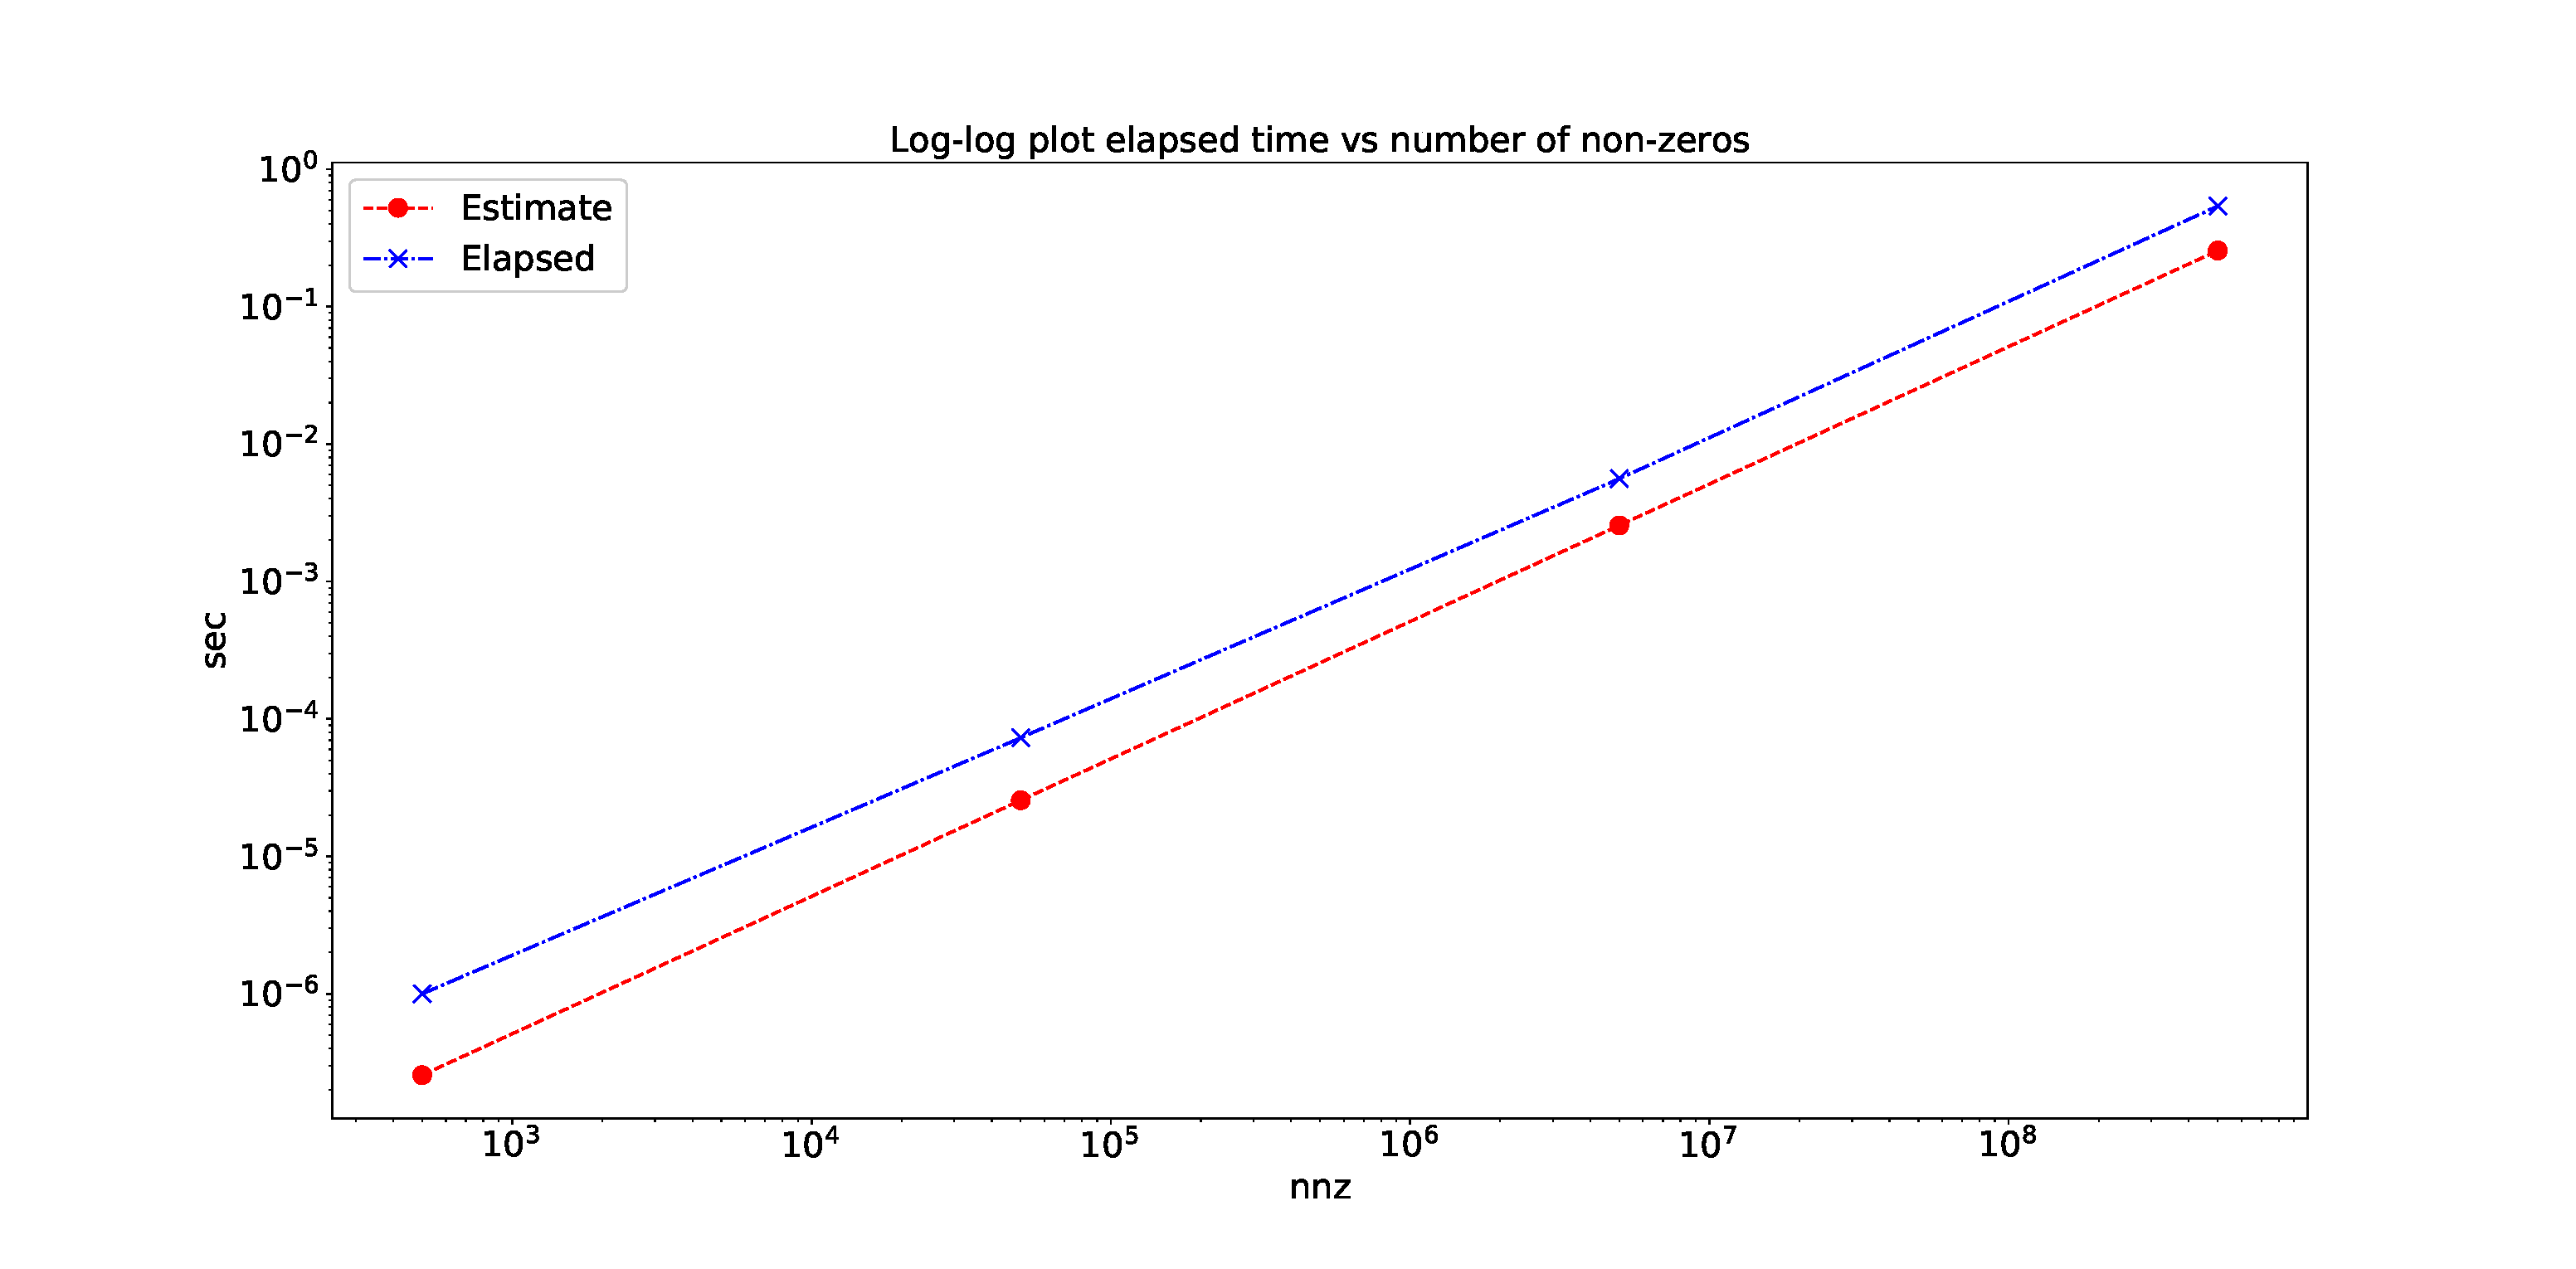
\includegraphics[scale=0.25]{nnz_time.eps}
        \captionsetup{width=.9\linewidth}
        \caption{Logarithmic plot of the elapsed time (estimate and actual) versus the number of non-zero elements in the matrix.}
        \label{nnz_vs_time}
    \end{figure}
    \item One important reason is that memory is \textbf{not} infinitely large or infinitely fast.
    \item Memory bandwidth (bits/seconds) is the hint (total number of bits loaded) divided by $t_\text{obs}$:
    \begin{itemize}
        \setlength\itemsep{0.01em}
        \item $\text{nrows} = 10^2 \Rightarrow 7046 \ \text{Gbit/s}$
        \item $\text{nrows} = 10^4 \Rightarrow 8310 \ \text{Gbit/s}$
        \item $\text{nrows} = 10^6 \Rightarrow 12341 \ \text{Gbit/s}$
        \item $\text{nrows} = 10^8 \Rightarrow 13320 \ \text{Gbit/s}$
    \end{itemize}
    \begin{figure}[ht!]
        \centering
        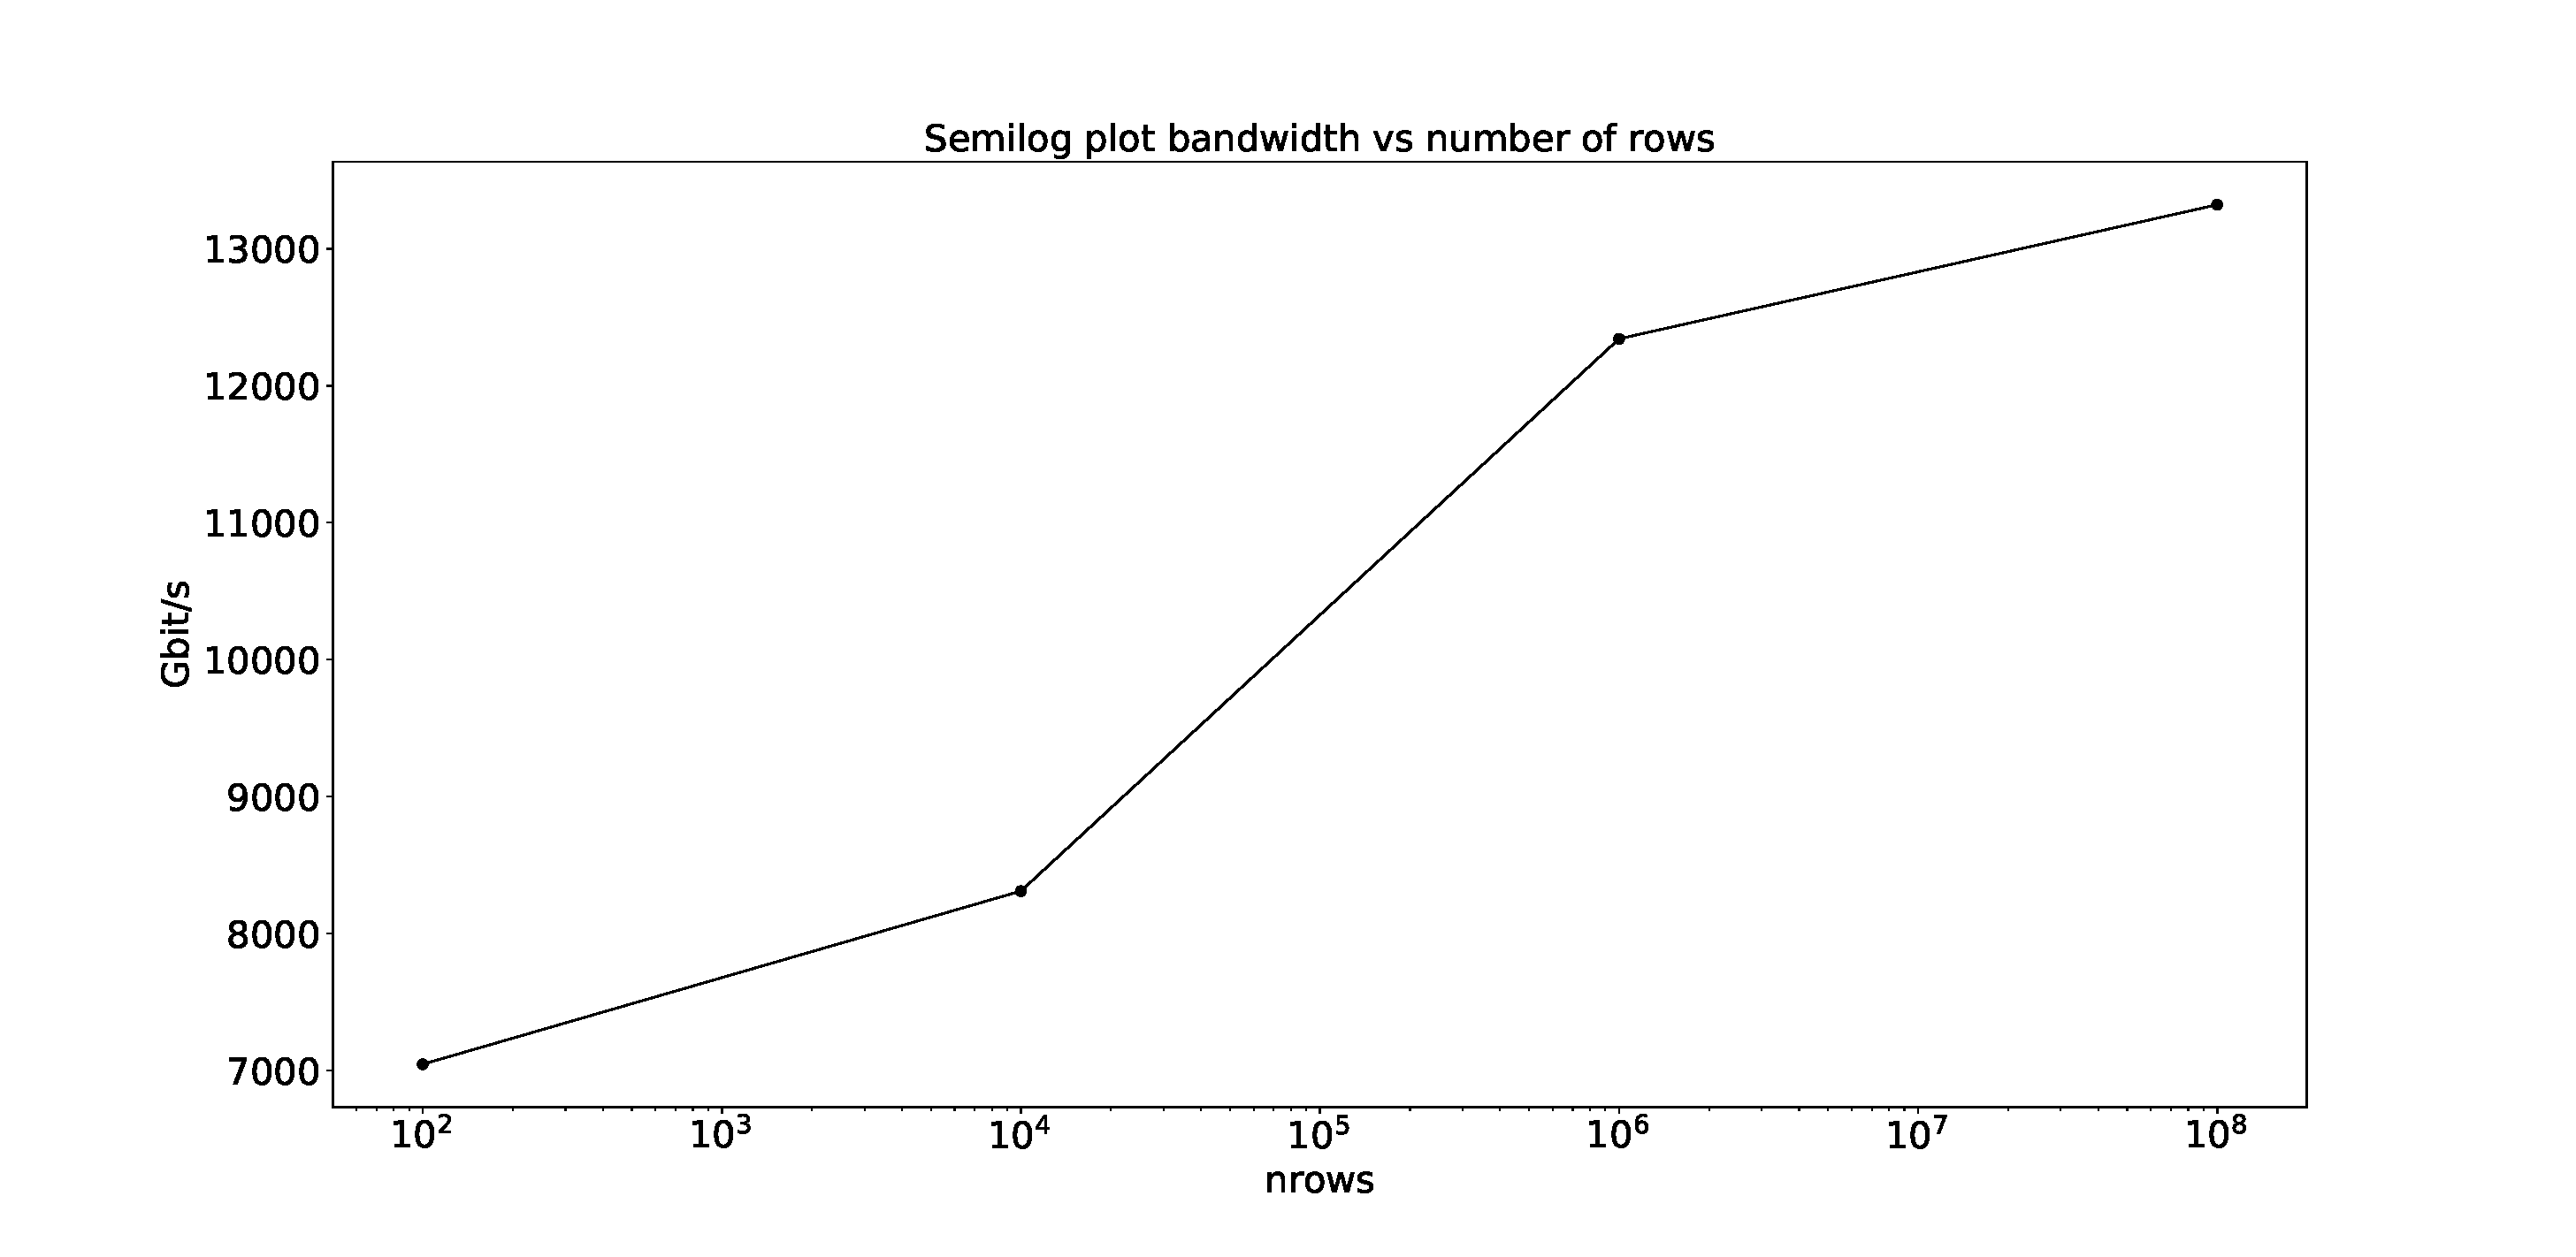
\includegraphics[scale=0.25]{nrows_band.eps}
        \captionsetup{width=.9\linewidth}
        \caption{Semi-logarithmic plot of the memory bandwidth versus the number of rows.}
        \label{nnz_vs_time}
    \end{figure}
    \item The bandwith obtained with the STREAM benchmark is only $\sim171 \ \text{Gbit/s}$ so there is a difference of a factor 50-100 (the numbers at question 4 are too high because they do not account for cache).
\end{enumerate}

\section{The memory mountain}

\begin{enumerate}
    \setlength\itemsep{0.01em}
    \item AMD Ryzen 7 3800x @ 3.9 GHz. L1 is 32 KB, L2 is 512 KB, L3 is 32 MB.
    \item See figure \ref{mountain}.
    \item An array size of 16 KB with a stride of 1-4 (x8 bytes). Bandwidth around 40 GB/s.
    \item An array size of 16-128 MB with a stride of 6-16 (x8 bytes). Bandwidth around 5 GB/s.
    \item Even though the larger array sizes indeed do not fit into (even) the L3 cache, a stride=1 still offers better performance because at smaller strides it is ``easier" for the prefetcher to guess which parts of the array are going to be needed in the future.
    \item Temporal locality: data is accessed (reused) by the CPU multiple times over a \textit{very short} time frame (i.a. local in time). Spatial locality: data that are stored relatively close together (e.g. two ints that are next to each other in an array are next to each other in memory). Locality is a desirable property as it provides a certain predictability that can exploited by CPU catching and prefetching to increase performance.
    \item Increased array size will decrease temporal locality because as you increase the array size, at a certain point it won't all fit in (the same level) cache anymore.
    \item Increased read stride will decrease spatial locality.
    \item We repeat the analysis on Beskow. The overall shape of the memory mountain remains qualitatively similar, however some interesting features can be spotted:
    \begin{itemize}
        \item while peak performance is still obtained around array sizes of 16KB and strides of 8 bites, now the plateau of lower performance is close to the maximum stride/size combination tested (32$\times$8 bites, 128MB);
        \item in general, performance for smaller sizes is higher and seems more consistent across different strides (less spikes due to noisy results).
    \end{itemize}
\end{enumerate}

\begin{figure}[ht!]
    \centering
    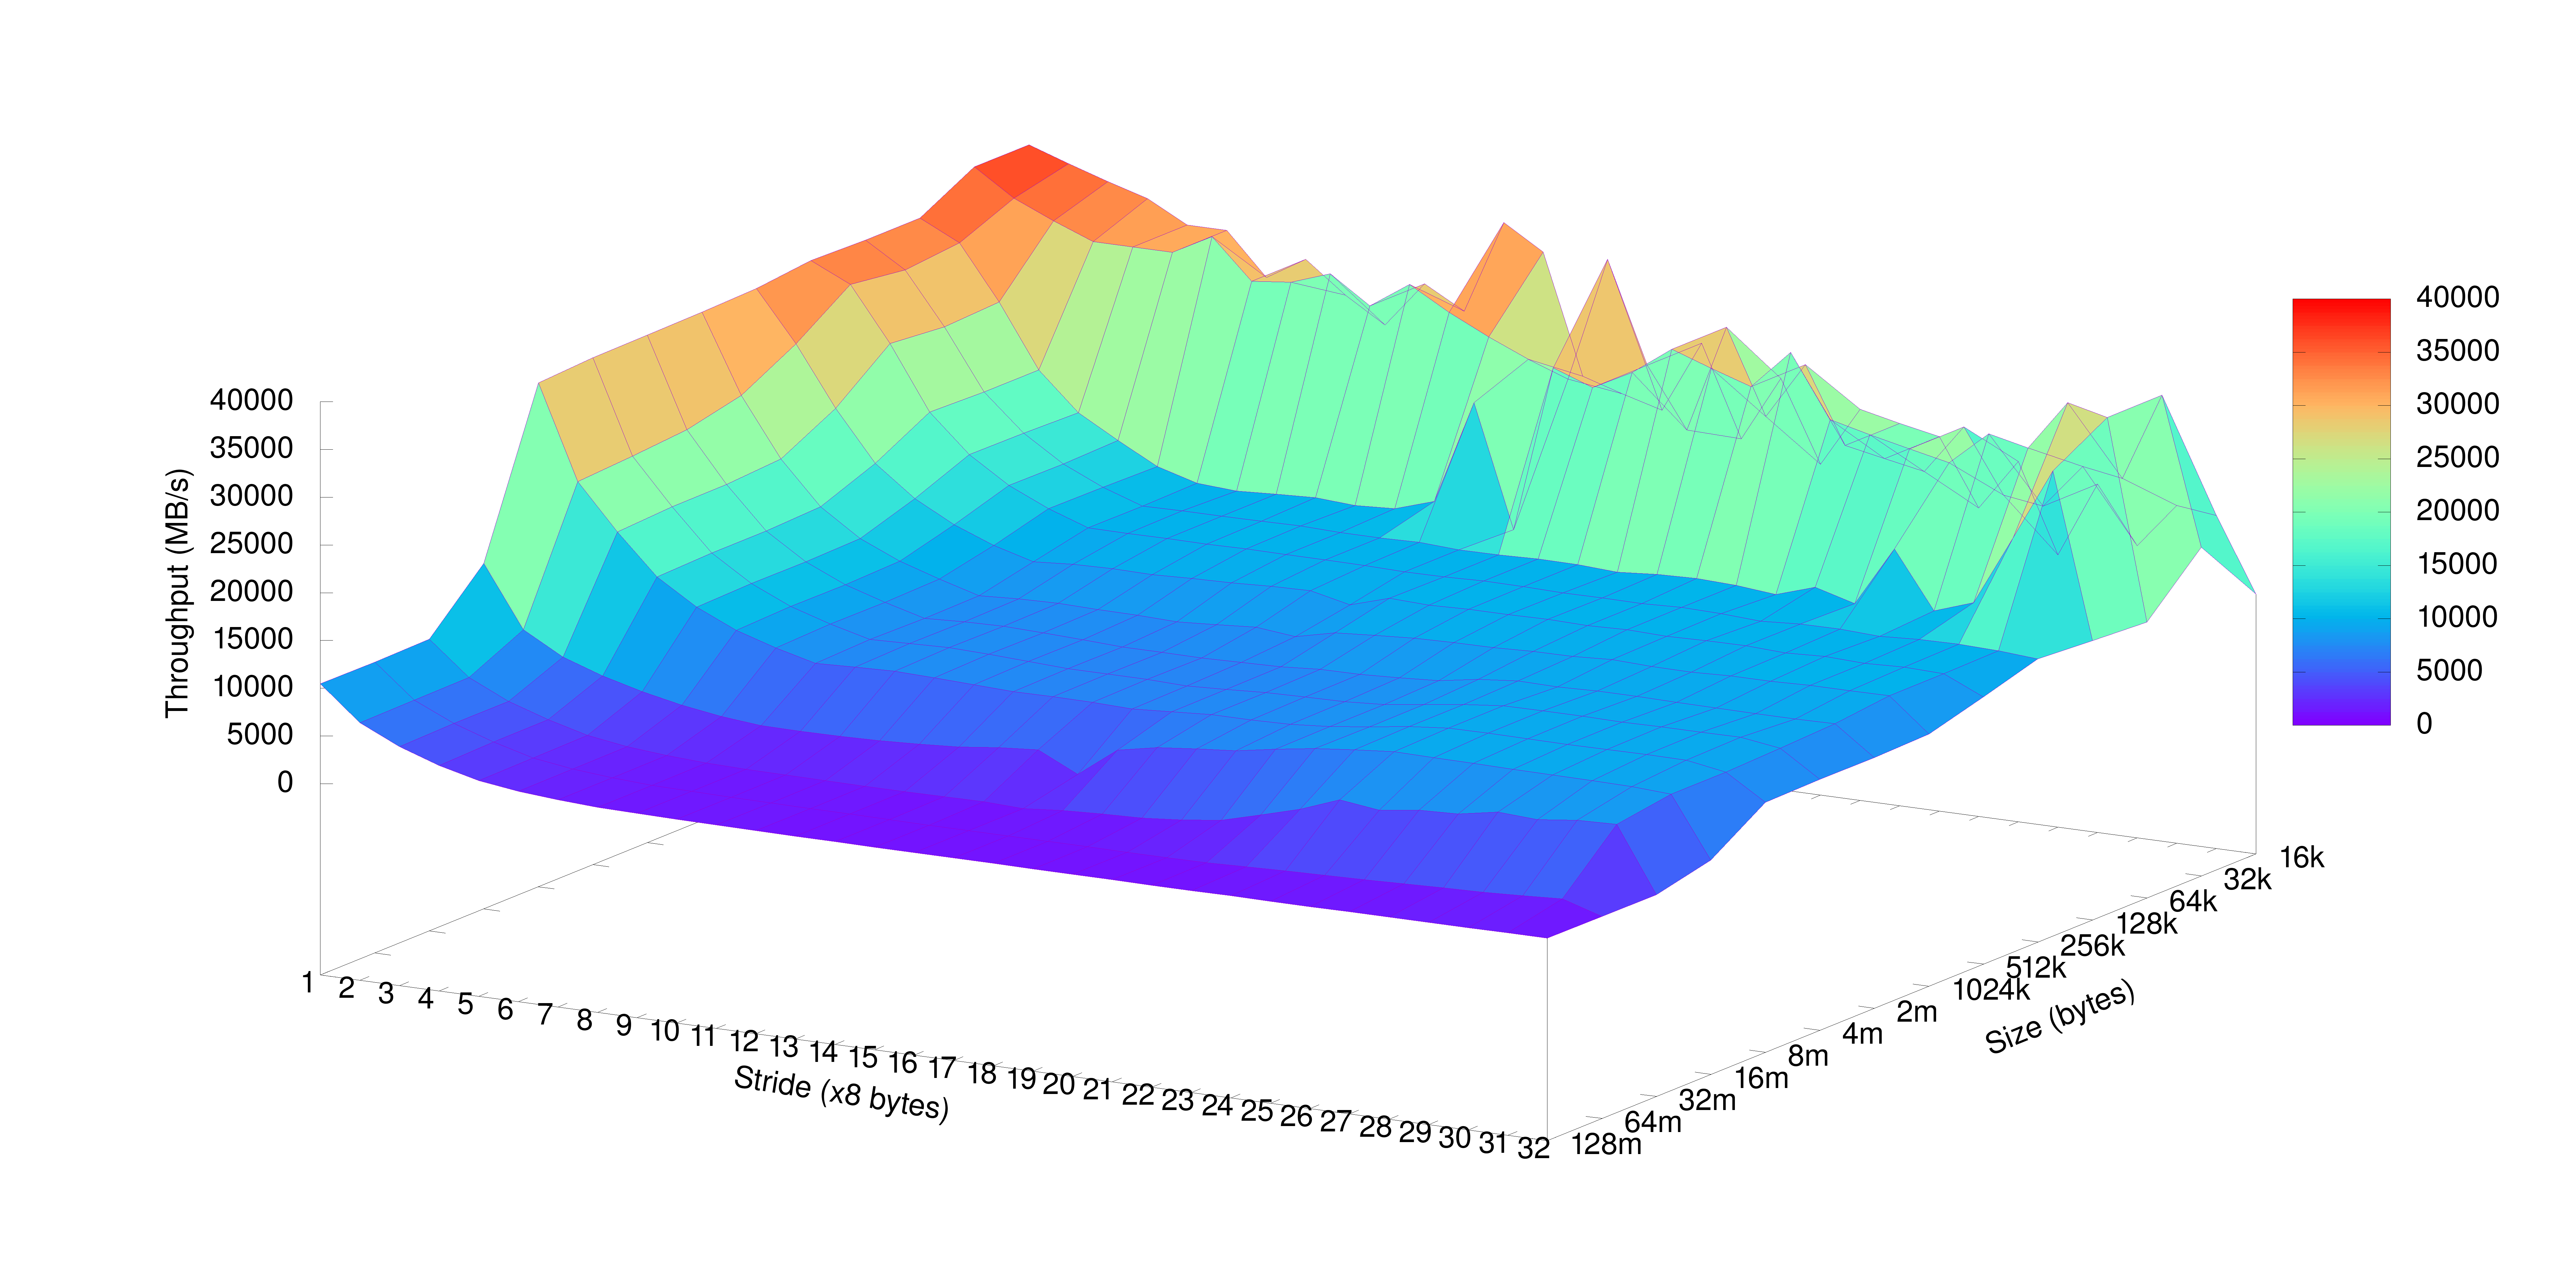
\includegraphics[scale=0.06]{memory_mountain.png}
    \captionsetup{width=.9\linewidth}
    \caption{The memory mountain for the AMD Ryzen 7 3800x. L1 is 32 KB, L2 is 512 KB, L3 is 32 MB.}
    \label{mountain}
\end{figure}

\begin{figure}[ht!]
    \centering
    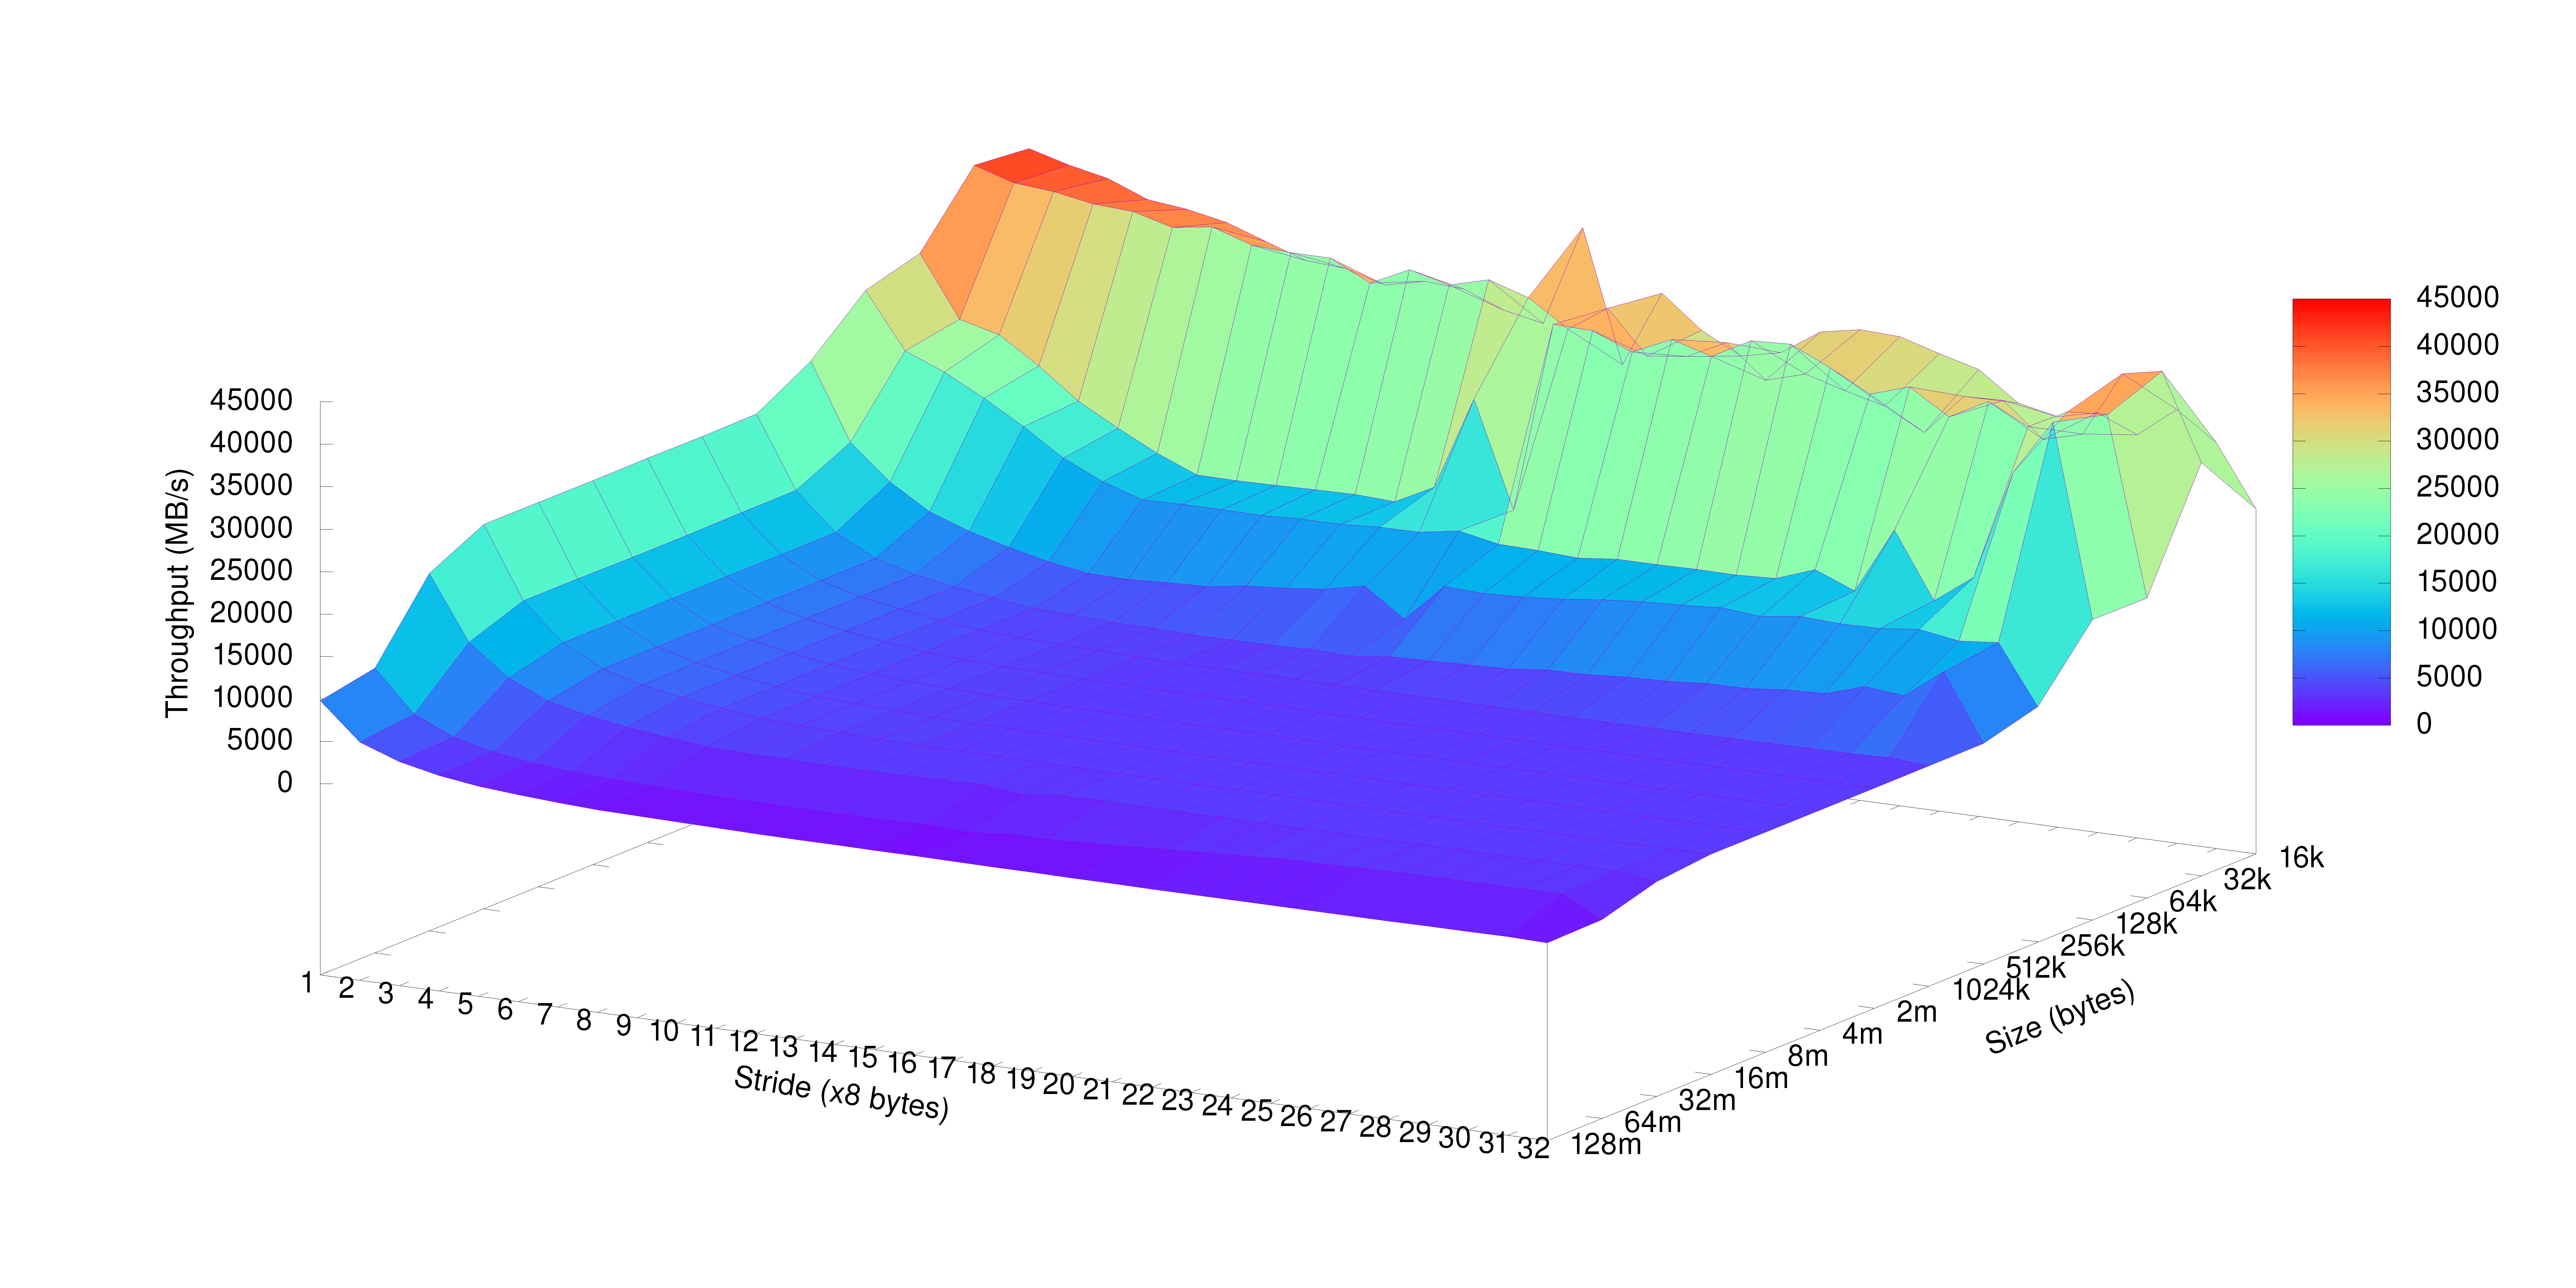
\includegraphics[scale=0.06]{memory_mountain_beskow.png}
    \captionsetup{width=.9\linewidth}
    \caption{The memory mountain obtained by running on Beskow (1 Haswell CPU, cache: L1 64KB, L2 256KB, L3 45MB).}
    \label{mountain_beskow}
\end{figure}

% {\color{red}[Maybe I can add the results from Beskow for point 9.]}

\section{Write a benchmark to measure performance}

\subsection{Compile the program with optimization flag \texttt{-O2} and execute it}

\begin{enumerate}
    \setlength\itemsep{0.01em}
    \item Average execution time is $9.5 \times 10^{-7} \ \text{s}$ (for N = 5000).
    \item For N = 100,000 the average execution time is still $9.5 \times 10^{-7} \ \text{s}$.
    \item Execution time is like that because the compiler is smart and sees that although we declare and initiate very large arrays, we don't actually use them for anything: the compiler therefore optimizes these instructions (essentially removes them). This can easily be verified by adding another \texttt{for} loop, outside the timed one, just for printing vector \texttt{c}: \texttt{t2-t1} increases now to $10^{-5}\div10^{-4}$ seconds. We can prevent the compiler from doing this by removing the \texttt{-O} (optimization level) flag, or setting the \texttt{-O0} flag (useful for debugging purposes).
    \item Execution time is $2 \times 10^{-5} \ \text{s}$ for N = 5000, and $2 \times 10^{-4} \ \text{s}$ for N = 100,000.
\end{enumerate}

\subsection{Check the tick (clock granularity) on Beskow or your local computer}

\begin{enumerate}
    \setlength\itemsep{0.01em}
    \item Clock granularity (local machine) is $9.54 \times 10^{-7} \ \text{s}$ (using clockgranularity.c).
    \item Theoretically, since we are directly measuring the amount of clock cycles for a certain operation, the granularity would be $1/\text{CPUspeed} = (3.9 \times 10^9 \ \text{Hz})^{-1} \approx 2.6\times 10^{-10} \ \text{s}$. However, measuring ``nothing at all" in the code already gives an average of 122.8 cycles, so we might need to subtract this when we bench an actual operation?
\end{enumerate}

\subsection{Modify the program in 1.1}

\begin{enumerate}
    \setlength\itemsep{0.01em}
    \item Average run time is now $2.4 \times 10^{-6} \ \text{s}$ for $N = 5000$, and $4.8 \times 10^{-5} \ \text{s}$ for $N = 100000$. Averaged over 100,000 runs.
\end{enumerate}

\newpage
\section{Measure the cache usage in matrix-matrix multiply}

We utilize PERF tool to monitor the performance of dense matrix-matrix multiplication code both on our local machine and on Beskow; in the latter case, the bash comand to run \texttt{perf} and store results is:\\
\\
\texttt{srun -n 1 perf stat -e instructions,cycles,L1-dcache-load-misses,L1-dcache-loads,} \\
\null\quad\texttt{LLC-load-misses,LLC-loads ./matrix\_multiply\_naive\_64.out > perf.out 2> perf.err}\\
\\
Results for elapsed time, instructions per cycle and cache misses is reported on table \ref{table:perf_laptop}, \ref{table:perf_beskow}.

\begin{table}
\begin{center}
\begin{tabular}{ r||c|c|c|c| } 
 \hline
 \textbf{Benchmark} & naive N=64 & naive N=1000 & optimized N=64 & optimized N=1000 \\
 \hline
 \hline
 \textbf{Elapsed} [sec]	& 0.002556 & 20.402589 & 0.001918 & 6.724911 \\
 \textbf{IPC} & 2.223877 & 1.088776 & 2.975347 & 2.936540 \\
 \textbf{L1 cache miss ratio} & 0.114576 & 0.609410	& 0.019447 & 0.062875 \\
 \textbf{L1 c. m. r. PTI} & 32.401968 & 174.017899 & 5.521993 & 17.959024 \\ 
 \textbf{LLC cache miss ratio} & 0.070411 & 0.249709 & 0.088393 & 0.231928 \\
 \textbf{LLC c. m. r. PTI} & 0.011512 & 4.830218 & 0.013629 & 0.160214 \\
 \hline
\end{tabular}
\caption{Dell laptop, Intel(R) Core(TM) i7-8565U CPU @ 1.80GHz, averaged over \texttt{-r 10} tests.}
\label{table:perf_laptop}
\end{center}
\end{table}

\begin{table}
\begin{center}
\begin{tabular}{ r||c|c|c|c| } 
 \hline
 \textbf{Benchmark} & naive N=64 & naive N=1000 & optimized N=64 & optimized N=1000 \\
 \hline
 \hline
 \textbf{Elapsed} [sec]	& 0.009906 & 18.106535 & 0.007400 & 5.845140 \\
 \textbf{IPC} & 1.241768 & 1.051635	& 1.951368 & 4.107198 \\
 \textbf{L1 cache miss ratio} & 0.077857 & 0.602505	& 0.024028 & 0.062764 \\
 \textbf{L1 c. m. r. PTI} & 30.049127 & 200.688763 & 8.736777	& 17.916551 \\ 
 \textbf{LLC cache miss ratio} & N/D & 0.000013 & N/D & 0.000103 \\
 \textbf{LLC c. m. r. PTI} & N/D & 0.000279	& N/D & 0.000059 \\
 \hline
\end{tabular}
\caption{Beskow, 1 Haswell CPU, average over \texttt{-r 5} tests.}
\label{table:perf_beskow}
\end{center}
\end{table}

The main factors hindering the performance of the matrix multiply could be summarized as follow.
\begin{itemize}
    \item C arrays are arranged in row-major order; the naive implementation fetches a value from a different row of \texttt{matrix\_b} at each inner-most loop iteration and therefore fails to keep spacial locality, making inefficient use of the L1 data cache; indeed, the L1 cache misses in the naive case are one order of magnitude larger than the ones in the optimized code.
    \item Temporal locality is not ensured in the case of multuplication of \textit{dense} matrices; in general we observe an higher miss ratio (both for L1 and LLC) for N=1000, regardless on optimization. Given the large amount of L3 cache on Haswell CPUs, we no not observe any LLC-miss in the N=64 case for the tests run on Beskow.
    \item Neither the naive code nor the presented optimized code utilize \textit{loop unrolling} tecniques; only one value of \texttt{matrix\_r} ir reused in each inner-loop iteration, leading to relatively inefficient cache usage.
\end{itemize}

\newpage
\section{Vectorization}

\begin{itemize}
    \setlength\itemsep{0.01em}
    \item To enable vectorization for \texttt{gcc}, one has to set the \texttt{-O2} flag and the \texttt{-ftree-vectorize} flag. Optionally, one can just set the \texttt{-O3} flag as this includes the \texttt{-ftree-vectorize} flag (among others).
    \item\sloppy To obtain a compiler report on vectorization, we set the \texttt{-fopt-info-vec} and \texttt{-fopt-info-vec-missed} flags. These will gives us reports on succesful and failed vectorization attempts, respectively.
    \item 
\begin{verbatim}
gcc -O3 -fopt-info-vec -fopt-info-vec-missed matrix_multiply.c
    -o matrix_multiply.out
\end{verbatim}

    \item Vectorization report for the command above:
\begin{verbatim}
matrix_multiply.c:18:19: missed: statement clobbers memory: gettimeofday (&tp, &tzp);
matrix_multiply.c:26:18: missed: couldn't vectorize loop
matrix_multiply.c:28:37: missed: statement clobbers memory: _1 = rand ();
matrix_multiply.c:27:20: missed: couldn't vectorize loop
matrix_multiply.c:28:37: missed: statement clobbers memory: _1 = rand ();
matrix_multiply.c:28:37: missed: statement clobbers memory: _1 = rand ();
matrix_multiply.c:29:37: missed: statement clobbers memory: _4 = rand ();
matrix_multiply.c:39:18: missed: couldn't vectorize loop
matrix_multiply.c:39:18: missed: not vectorized: multiple nested loops.
matrix_multiply.c:40:20: optimized: loop vectorized using 16 byte vectors
matrix_multiply.c:41:22: missed: couldn't vectorize loop
matrix_multiply.c:41:22: missed: outer-loop already vectorized.
matrix_multiply.c:52:18: missed: couldn't vectorize loop
matrix_multiply.c:54:27: missed: not vectorized: complicated access pattern.
matrix_multiply.c:53:20: optimized: loop vectorized using 16 byte vectors
matrix_multiply.c:52:18: missed: couldn't vectorize loop
matrix_multiply.c:54:27: missed: not vectorized: complicated access pattern.
matrix_multiply.c:53:20: optimized: loop vectorized using 16 byte vectors
matrix_multiply.c:71:17: missed: couldn't vectorize loop
matrix_multiply.c:71:17: missed: not vectorized: multiple nested loops.
matrix_multiply.c:39:18: missed: couldn't vectorize loop
matrix_multiply.c:39:18: missed: not vectorized: multiple nested loops.
matrix_multiply.c:40:20: optimized: loop vectorized using 16 byte vectors
matrix_multiply.c:41:22: missed: couldn't vectorize loop
matrix_multiply.c:41:22: missed: outer-loop already vectorized.
matrix_multiply.c:39:18: missed: couldn't vectorize loop
matrix_multiply.c:39:18: missed: not vectorized: multiple nested loops.
matrix_multiply.c:40:20: optimized: loop vectorized using 16 byte vectors
matrix_multiply.c:41:22: missed: couldn't vectorize loop
matrix_multiply.c:41:22: missed: outer-loop already vectorized.
\end{verbatim}

    If we look at the report, there are two reasons why 
    vectorization fails, either:

    \begin{itemize}
        \setlength\itemsep{0.01em}
        \item there are  multiple (more than two) nested loops,
        \item the access pattern is too complicated.
    \end{itemize}

    Both boil down to the fact that for complicated situations (e.g. vectorization of non-primitive types) the compiler simply does not know how to do it and/or the architecture does not allow it.
\end{itemize}

% \section{Bibliography}
% \printbibliography[heading=none]

\end{document}
